\section{Evaluation}

This section answers the following questions experimentally:
\begin{CompactItemize}
\item Does \ldu's design matter for applications?

\item Why does \ldu's scheme scale well?
\end{CompactItemize}


\subsection{Experimental setup}


\subsection{AIM7}


%$$$$$$$$$$$$$$$$$$$$$$$$$$$$$$$$$$$$$$$$$$$$$$$$$$$$$$$$$$$$$$$$$$$$$$$$$$$$$$$$
%Reference Sentence 1
%$$$$$$$$$$$$$$$$$$$$$$$$$$$$$$$$$$$$$$$$$$$$$$$$$$$$$$$$$$$$$$$$$$$$$$$$$$$$$$$$






%$$$$$$$$$$$$$$$$$$$$$$$$$$$$$$$$$$$$$$$$$$$$$$$$$$$$$$$$$$$$$$$$$$$$$$$$$$$$$$$$
%Reference Sentence 2
%$$$$$$$$$$$$$$$$$$$$$$$$$$$$$$$$$$$$$$$$$$$$$$$$$$$$$$$$$$$$$$$$$$$$$$$$$$$$$$$$

%This section answers the following questions experimentally:

%\begin{CompactItemize}
%\item Does \deferu's design matter for applications?

%\item Why does \deferu's scheme scale well?
%\end{CompactItemize}


% AIM7, EXIM, Lmbench



% Dynamic nonblocking and lock-less data strucures(structures that access
% dynamically allocated memory that may also be freed at runtime) must typically
% rely on alternative safe memory recalamation mechanisms[COMMUNICATION of the
% ACM 2013] .

%We implemented the new deferred update algorithm in Linux 3.19.rc4 kernel, and
%our modified Linux is available as open source.
%\deferu's scheme is based on deferred processing, so it needs a garbage
%collector for delayed free.
%In order to implement the garbage collector, we use the lock-less list and a
%periodic timer(1 sec) in the Linux.

%Paragraph 2: 문제점을 해결하기 위해 Harris linked list를 적용
%We compare our \deferu implementation to a concurrent non-blocking Harris
%linked list ~\cite{Harris2001Lockfree};therefore, we implement the Harris
% linked list to Linux kernel.
%The code refers from sysnchrobench~\cite{Gramoli2015Synchrobench} and
%ASCYLIB~\cite{David2015ASYNCHRONIZED}, and we convert their linked list to
%Linux kernel style.
%Because both synchrobench and ASCYLIB leak memory, we implement additional
%garbage collector for the Linux kernel using Linux's work queues and lock-less
%list.

%Paragraph 3: 오브젝트의 특징을 고려한 lock-free list 구현 
%In order to further improve performance, we move their ordered list to
%unordered list. 
%A feature of the Harris linked list is all the nodes are ordered by
%their key. 
%Zhang~\cite{zhang2013practical} implements a lock-free unordered list
%algorithm, whose list is each insert and remove operation appends an
%intermediate node at the head of the list;these approach is practically
%hard to implement.
%Indeed, Linux does not require contains operation because the Linux data
%structures such as list, tree and hash table not depended on search key;they
%depend on their unique object.
%This feature can eliminates the ordered list in Harris linked list.
%Therefore, we perform each insert operation appends an intermediate node at
%the first node of the list;on the other hand, each remove operation searches
%from head to their node.

%Paragraph 4: mapping은 DeferU와 Harris linked 리스트 둘 다 적용, 
%하지만 anon은 Harris Lined list 만 적용과 이유
%To the scalability of fork, the reverse mapping's lock contention should
%be eliminated not only from file reverse mapping but also from anonymous
% reverse mapping.
%The structure of file reverse mapping is simplified relatively to the
%structure of anonymous mapping because the anonymous reverse mapping is
%entangled by their global object(\code{anon\_vma}) and their
%chain(\code{anon\_vma\_chain});therefore, we only apply \deferu to file reverse
%mapping.



%\subsection{Experimental setup}
%Paragraph 1: 벤치 마크 대한 설명
%To evaluate the performance of \deferu, we use well-known
%three benchmarks:AIM7 Linux scalability benchmark, Exim email server in
%MOSBENCH and lmbench.
%We selected these three benchmarks because they are fork-intensive workloads
% and exhibit high reverse mapping lock contentions.
%Moreover, AIM7 benchmark has widely been used in practical area not only for
% testing the Linux but also for improving the scalability. 
%To evaluate \deferu for real world
%applications, we use Exim which is the most popular email server.
%A micro benchmark, Lmbench, has been selected to focus on Linux fork
% operation-intensive fine grained evaluations.
%Finally, we wanted to focus on Linux fork performance and scalability;therefore,
%we selected lmbench, a micro benchmark.

%Paragraph 2: 비교 대상에 대한 설명
%In order to evaluate Linux scalability, we used four different experiment
%settings.
%First, we used the stock Linux as the baseline reference. 
%Second, we used ordered Harris lock-free list while 
%we apply unordered Harris lock-free list for the third setting
%(see section ~\ref{sec:implementation}). 
%Finally, we used combination of unordered Harris lock-free list for anonymous
% mapping and our \deferu for file mapping.
%Since we cannot obtain detailed implementation of Oplog, 
%we could not include comparison between \deferu and Oplog in this paper.
%In fact, Oplog's design is based on per-core processing for update-heavy
%structure, but we cannot acquire their detail implementation;therefore, we
%evaluated these four combination.

%Paragraph 3: 운영체제 및 커널 버전 설명
%We ran the three benchmarks on Linux 3.19.rc4 with stock Linux with 
%the automatic NUMA balancing feature disabled because the
%Harris linked list has the iteration issue~\cite{petrank2013lock}. 
%All experiments were performed on a 120 core machine with 8-socket, 15-core
%Intel E7-8870 chips equipped with 792 GB DDR3 DRAM.

%\subsection{AIM7}
%Figure : AIM7 실험 결과

%\begin{figure}[tb]
%  \begin{center}
%    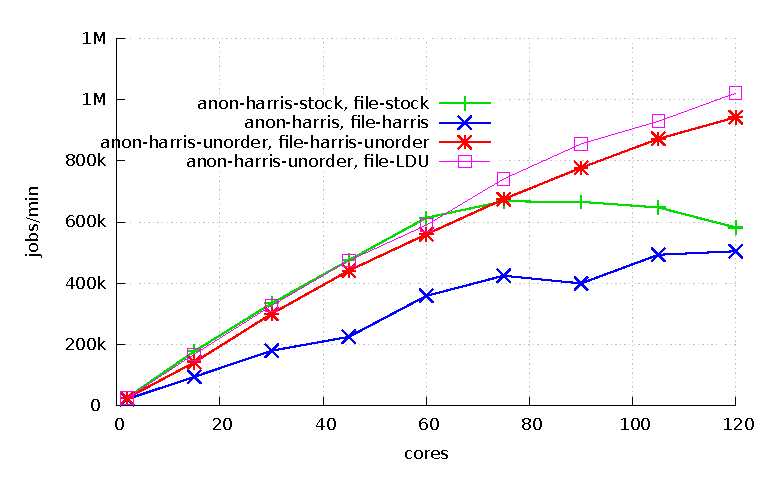
\includegraphics[scale=0.65]{graph/aim7.eps}
%  \end{center}
%  \caption{Scalability of AIM7 multiuser for different method.  The combination
%  \deferu with unordered harris list scale well;in contrast, up to 60 core, the
%  stock Linux scale linearly, then it  flattens out.}
%  \label{fig:aim7}
%\end{figure}

%Paragraph 1: 워크로드에 대한 설명
%AIM7 forks many processes, each of which concurrently runs. 
%We used AIM7-multiuser, which is one of workload in AIM7.
%The multiuser workload is composed of various workloads such as disk-file
%operations, process creation, virtual memory operations, pipe I/O, and
%arithmetic operation.
%To minimize IO bottlenecks, the workload was executed with tmpfs filesystems,
% each of which is 10 GB.
%To increase the number of users during our experiment and show the results at
% the peak user numbers, 
%we used the crossover.

%Paragraph 2: 실험 결과에 대한 설명
%The results for AIM7-multiuser are shown in Figure~\ref{fig:aim7}, and the
%results show the throughput of AIM7-multiuser with four different settings.
%Up to 60 core, the stock Linux scales linearly while serialized updates in
%Linux kernel become bottlenecks. 
%However, up to 120core, unordered harris list and our \deferu scale well
% because these workloads can run concurrently updates and can reduce the locking
%overheads due to reader-writer semaphores(\code{anon\_vma},
%\code{file}).
%The combination of \deferu with unordered harris list has best performance and
%scalability outperforming stock Linux by 1.7x and unordered harris list by
%1.1x.
%While the unordered harris list has 19\% idle time(see
%Table~\ref{tab:memuse}), stock Linux has 51\% idle time waiting to acquire
%both \code{anon\_vma's rwsem} and \code{file's i\_mmap\_rwsem}.
%We can notice that although \deferu has 23\% idle time, the throughput is
% higher than unordered harris list.
%In this benchmark, the ordered harris list has the lowest performance and
%scalability because their \code{CAS} fails frequently.

%\subsection{Exim}
% EXIM 실험 결과
%\begin{figure}[tb]
%  \begin{center}
%    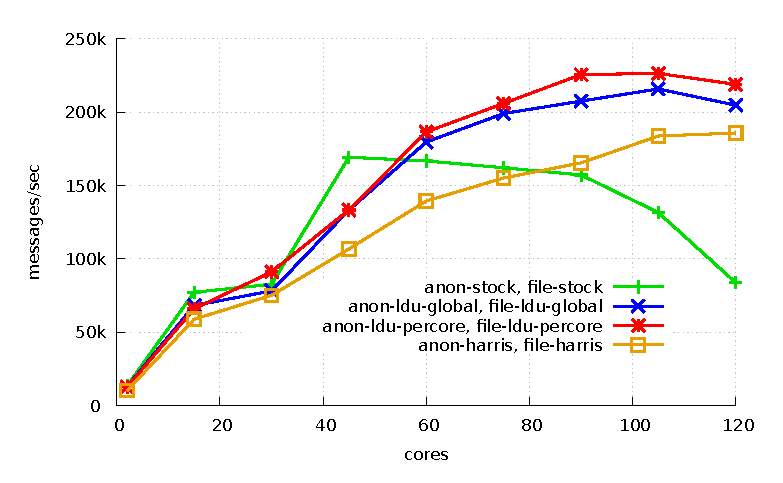
\includegraphics[scale=0.65]{graph/exim.eps}
%  \end{center}
%  \caption{Scalability of Exim. The stock Linux collapses after 60 core;in
%  contrast, both unordered harris list and our \deferu flatten out.}
%  \label{fig:exim}
%\end{figure}

%\begin{table}
%  \centering
%  \small
%  \begin{tabular}{l r r r } \toprule
%    AIM7 & user & sys & idle \\
%    \midrule
%    Stock(anon, file) & 2487 s & 1993 s & 4647 s(51\%)\\ 
%    H(anon, file) & 1123 s & 3631 s & 2186 s(31\%)\\
%    H-unorder(anon, flie) & 3630 s & 2511 s & 1466 s(19\%)\\
%    H-unorder(anon), L(file) & 3630 s & 1903 s & 1662 s(23\%)\\
%    \bottomrule
%  \end{tabular}
%  \begin{tabular}{l r r r } \toprule
%    EXIM & user & sys & idle \\
%    \midrule
%    Stock(anon, file) & 41 s & 499 s & 1260 s(70\%)\\ 
%    H(anon, file) & 47 s & 628 s & 1124 s(62\%)\\
%    H-unorder(anon, file) & 112 s & 1128 s & 559 s(31\%)\\
%    H-unorder(anon), L(file) & 87 s & 1055 s & 657 s(37\%)\\
%    \bottomrule
%  \end{tabular}
%  \begin{tabular}{l r r r } \toprule
%    lmbench & user & sys & idle \\
%    \midrule
%    Stock(anon, file) & 11 s & 208 s & 2158 s(91\%)\\ 
%    H(anon, file) & 11 s & 312 s & 367 s(53\%)\\
%    H-unorder(anon, file) & 11 s & 292 s & 315 s(51\%)\\
%    H-unorder(anon), L(file) & 12 s & 347 s & 349 s(49\%)\\
%    \bottomrule
%  \end{tabular}

%  \caption{Comparison of user, system and idle time at 120 cores.}
%  \label{tab:memuse}
%\end{table}


%Paragraph 1: 워크로드에 대한 설명
%To measure the performance of Exim, shown in Figure~\ref{fig:exim}, we
%used default value of MOSBENCH to use tmpfs for
%spool files, log files, and user mail files.
%Clients run on the same machine and each client sends to a different user to
%prevent contention on user mail file.
%The Exim was bottlenecked by per-directory locks protecting file creation in
%the spool directories and by forks performed on different
%cores~\cite{SilasBoydWickizer2010LinuxScales48}.
%Therefore, although we eliminate the fork problem, the Exim may suffer from
%contention on spool directories. 

%Paragraph 2:실험 결과에 대한 설명
%Results shown in Figure~\ref{fig:exim} show that Exim scales well for all
%methods up to 60 core but not for higher core counts.
%The stock Linux shows performance degradation for more than 60 core.
%Both unordered harris list
%and our \deferu do not suffer from performance loss 
%because they do not acquire the \code{anon\_vma}
%semaphore and \code{i\_mmap} semaphore in fork.
%\deferu performs better due to the fact that it uses both update-side
%absorbing and lock-less list, outperforming stock Linux by 1.6x and unordered
%harris list by 1.1x.
%Even though we applied scalable solution, Exim shows limitation on scalability
%improvement
%since the main bottleneck is per-directory lock contention on spool
%directories.
%The unordered harris list has 31\% idle time, whereas \deferu has 37\% idle
%time due to the their efficient concurrent updates.

%\subsection{lmbench}
%\begin{figure}[tb]
%  \begin{center}
%    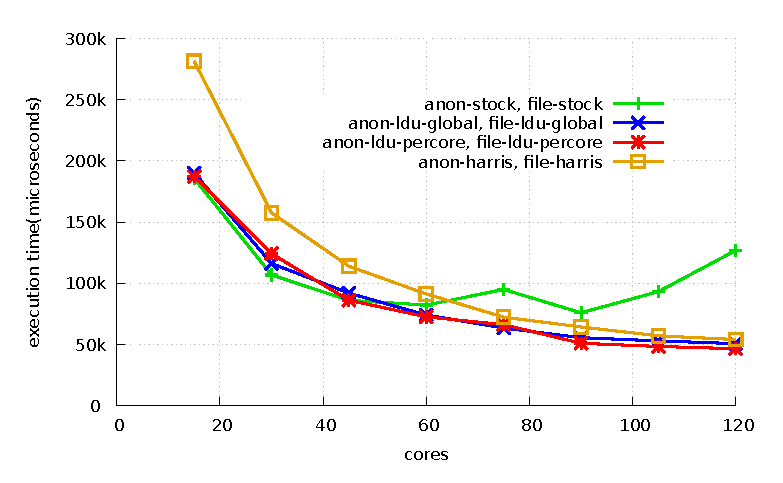
\includegraphics[scale=0.65]{graph/lmbench.eps}
%  \end{center}
%  \caption{Execution time of lmbench's fork micro benchmark. The fork micro
%  benchmark drops down for all methods up to 15 core but either flattens out or
%  goes up slightly after that. At 15 core, the stock Linux goes up;the others
%  flattens out}
%  \label{fig:MicroBench}
%\end{figure}

%Paragraph 1: %워크로드에 대한 설명
%lmbench has various workloads including process creation workload(fork,
%exec, sh -c, exit).
%This workload is used to measure the basic process primitives such as creating
%a new process, running a different program, and context switching. 
%We configured process create workload to enable the parallelism option which
%specifies the number of benchmark processes to run in
%parallel~\cite{mcvoy1996lmbench}; we used 100 processes.

%Paragraph 2: 실험 결과에 대한 설명
%The results for lmbench are shown in Figure~\ref{fig:MicroBench}, 
%and the results show the execution times of the fork microbenchmark in lmbench
%with four different methods.
%The fork micro benchmark drops down for all methods up to 15 core but either
%flattens out or goes up slightly after that.
%Three methods outperform stock Linux by 2.2x at 120 cores;however, before 30
%core, two harris list have lower performance due to their execution overheads.
%At 15 core, the stock Linux goes up because of the NUMA effect that accesses
%the remote memory.
%On the other hand, the others including the ordered harris list flattens out
%and then they remain constant.
%While stock Linux has 90\% idle time, other methods have approximately 50\%
%idle time since stock Linux waits to acquire reverse mapping locks such as
%\code{anon\_vma's rwsem} and \code{mapping's i\_mmap\_rwsem}.
